\Section{Off-chain atomic swaps}
Atomic swaps over a payment channel is possible, often refered to as offchain atomic swap. The mechanisms that makes it work may not be as clear as one that takes place entirely onchain. 

To clear some things up before moving on: \textbf{both} parties that are performing the swap needs to have a functioning node on the respective networks of the cryptocurrencies to be exchanged. The channels do \textbf{not} need to be directly connected to each other instead they can take any route through both networks, given that the route allows the exchanged amount of course.

If we say that Alice (A) and Bob (B) want to do an offchain atomic swap, Alice has bitcoins and wants litecoins, Bob has litecoins and wants bitcoins. Let's also say that Alice is the one that initiates the swap (meaning that in this case she sends the initial transaction). An offchain atomic swap can be thought of as a transaction that propagates through both the networks. Alice sends a transaction to Bob on the bitcoin network, Bob re-sends a transaction with the same pre-image hash on the litecoin netowrk to Alice. The timelocks are set so that the time continually decreases (like it would on a regular network transaction), even as it transitions into the litecoin network. Let's say that there are $m$ jumps between Alice and Bob on the bitcoin network and $n$ jumps between them on the litecoin network, and that each step needs at least 24 hours more to claim for each step. 

The timelock on the initial channel jump (the one Alice sends initially) would be:
$$(m+n+1) * 24h$$

When the transaction reaches Bob the timelock should be: 
$$(n+1) * 24h$$

This is where the swap differs from a normal transaction. In a regular transaction Bob would be the holder of the pre-image, and thus the pre-image could properly propagate backwards in the transaction chain from here. But in this case he does not know the pre-image and thus is forced to continue the chain on the litecoin chain if he ever wants to claim his bitcoins. As mentioned he sends the agreed upon litecoins to Alice via the litecoin network, still using the same pre-image hash used by Alice. He also continues with the same decreasing timelock (thus the next transaction will have a timelock of ($(n+1 - 1) * 24h$)

When the transaction on the litecoin network at last arrives to Alice the timelock should be set to:
$$(1) * 24h$$

When the litecoin transaction reaches Alice the circle is closed and Alice can safely reveal the pre-image. Every one in the transaction chain gets their rightful money. When the pre-image reaches Bob he has to propagate it backwards on the bitcoin network until it reaches Alice again. Just as with regular multi-hop transactions each channel is expected to settle without closing and spening the HTLC-ouput unless neccessary due to uncooperative nodes etc... 

As long as the same pre-image is used and the timelocks decrease monotonically across the networks this should be a safe swap. If let's say Bob tries to cheat Alice by not sending the agreed upon amount of litecoins Alice simply has to never reveal the pre-image anyone in the chain. Then all multi-hop transactions on both chains will have to be reset after the timelocks have expired.

\begin{figure}[H]
	\centering
	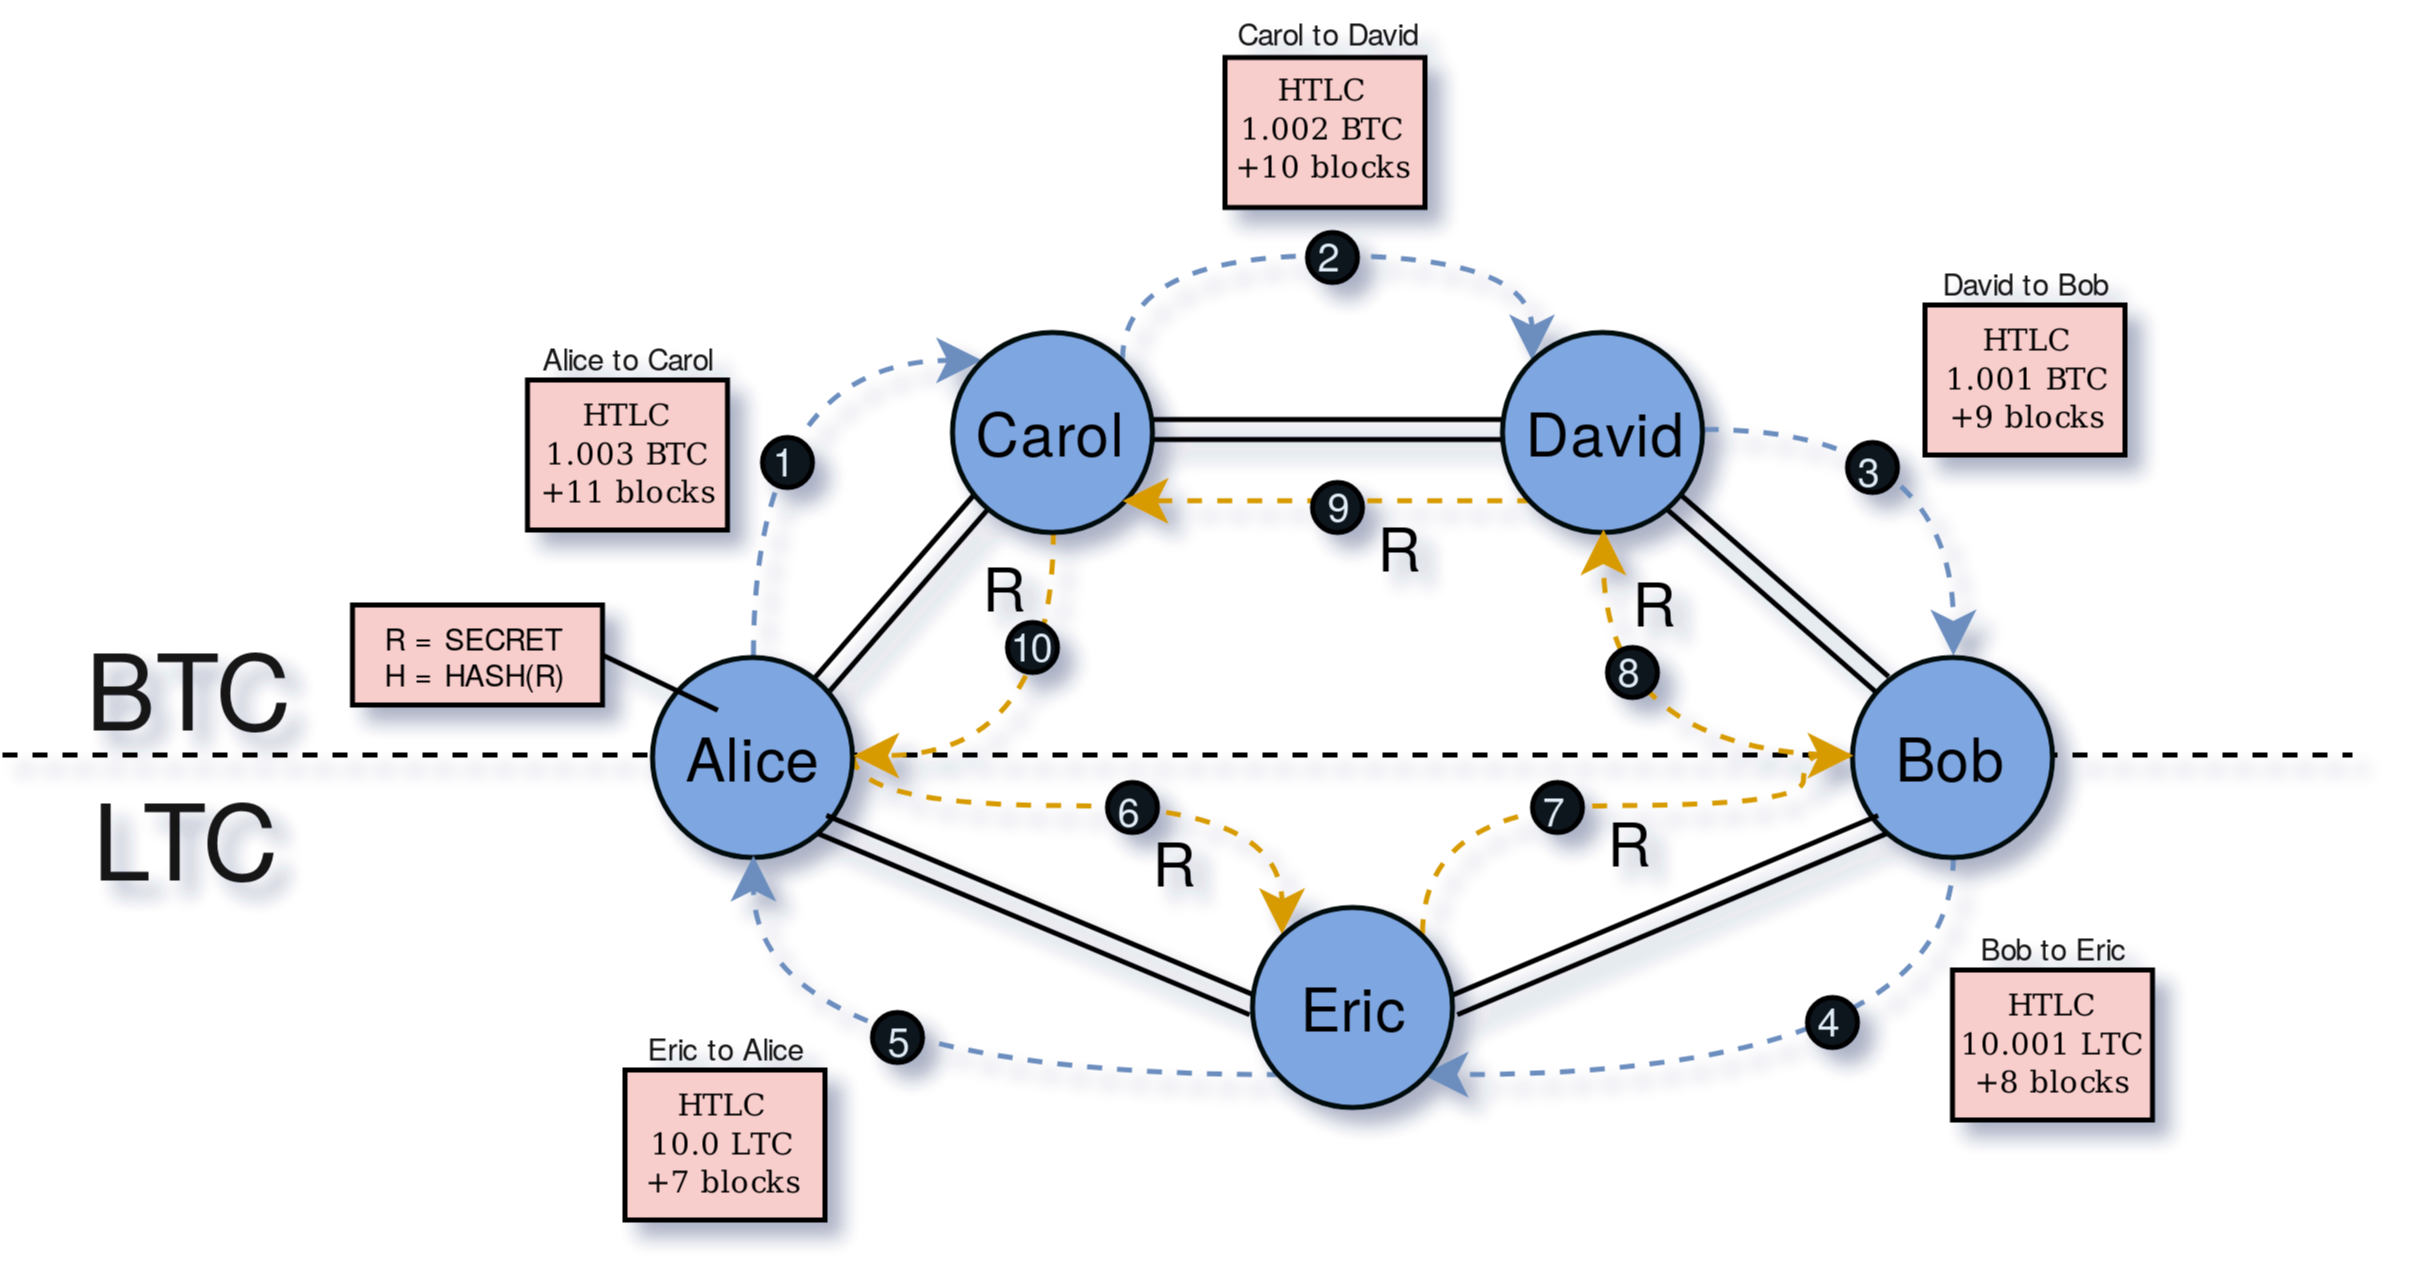
\includegraphics[width=1\textwidth]{background/images/ln_route_swap.png}
	\caption{Route taken by the multi-hop transactions on both networks. Note that Alice and Bob has a node in both the BTC and LTC network.}
	\label{fig:ln-swap}
\end{figure}

Figure \ref{fig:ln-swap} shows a rough diagram of the process. Alice and Bob has an active node in both the networks, no such assumption is needed for the other participants on either side. As mentioned the transaction could pass as many intermittent nodes as needed on either network, to keep the diagram small only two additional jumps are made on the Bitcoin side, and only one extra jump on the litecoin network.  

So to summarize the process: 

Alice and Bob agrees on doing a swap, they agree to exchange 1 bitcoin for 10 litecoins. Alice creates a new secret R and a new hash H = HASH(R). Sends a offchain transaction to Bob on the bitcoin network that gives him 1 bitcoin if he can provide the pre-image to H (R) (Steps 1 - 3 in the diagram). Bob sends a multi-hop transaction to Alice on the litecoin network, that gives Alice 10 litecoins if she can provide the pre-image to H (Steps 4 - 5 in the diagram). It is very important that the decreasing timelock that was used on the bitcoin side continues on the litecoin side. Otherwise the safety of the swap is not guaranteed. 

When Alice receives the litecoin transaction, she can safely reveal R to Eric, Eric will do the same to Bob. The R will travel backwards in the transaction chain just like with a regular lightning network transaction, but this time when the pre-image reaches Bob he will keep transmitting it backwards through the chain on the bitcoin network. (Steps 6 - 10 in the diagram).

\Subsection{Safety}
The way safety is assured in offchain atomic swaps is the same mechanisms that makes lightning network it self safe, which in turn is largely based on the mechanisms of the onchain atomic swap. 
Let's take a look at a couple of scenarios where malicious actors try to claim money that is not theirs. Using the general scenario shown in figure \ref{fig:ln-swap}.

\Subsubsection{Bob does not send his litecoins to Alice after receiving bitcoins}
This would be after step 3 in the diagram. At first it may seem that Bob will get his bitcoins after all, but Alice simply has to never reveal the pre-image R. The HTLC contract states that everyone along the chain can only claim their money if they can reveal the pre-image to the hash H. If Alice never reveals it, Carol, David and Bob will not be able to claim the money. In the optimal case no channel will have to close in this scenario, after the timelock has expired nobody on the chain has any reason not to amend the previous commit with HTLC with a new commit with the transactions revered. In the worst case, meaning that everybody refuses to cooperate, all the channels on the BTC side of the diagram has to be closed. The transaction reversal will be reflected on in the money that is now claimable onchain.

In both the worst and best case no monetary loss has occurred for any of the participants in the network.

\Subsubsection{Alice tries to claim the litecoins without revealing the pre-image to Eric}
In this case she will be able to claim her litecoins. But claiming them onchain will also reveal the secret R publicly on the blockchain. Even if Alice waited until just before the timelock expired to claim her litecoins, in this case 6 blocks, there is still time over for Eric to claim his litecoins on the Bob channel as that channel has a larger timelock. In the best case scenario only the channel between Alice and Eric is closed, while the rest settles normally (in this case in favor of the transaction). In the worst case all channels will have to be closed. Even so nobody will lose out on their share of the money as the timelock is ever increasing when going backwards in the payment chain, and for each step on the way the pre-image will be revealed on the blockchain just as it did between Alice and Eric. 

\Subsubsection{Somebody along the path stops cooperating}
Let's say Eric did not forward the transaction to Alice. This is just a variation of the first scenario. If Alice sees that something is wrong she will simply not reveal the pre-image to anyone and all channels will have to revert to previous state or be closed.